\documentclass[a4paper, 12pt]{report}

\usepackage[utf8x]{inputenc}
\PrerenderUnicode{ăîșțâĂÎÂȘȚ„”}
\usepackage{indentfirst}
\usepackage{bookman}
\usepackage[T1]{fontenc}
\usepackage{graphicx}
\usepackage{amsmath,amssymb}
\usepackage{siunitx}
\usepackage{mathtools}
\usepackage{subfig}
\usepackage{listings}
\usepackage{fancyhdr}
\usepackage{color}
\usepackage{courier}
\usepackage{float}
\usepackage{ifthen}
\usepackage{geometry}
\usepackage{booktabs}
\usepackage[table,xcdraw]{xcolor}
\usepackage[hidelinks,unicode]{hyperref}
\usepackage[bottom]{footmisc}

\usepackage{longtable}
\usepackage[nottoc]{tocbibind}
\usepackage{url}
\def\UrlBreaks{\do\/\do-}

\graphicspath{ {fig/} }

\pagestyle{fancy}
\fancyhead[RO]{\footnotesize{\thepage}}
\fancyhead[LO]{\footnotesize{\rightmark}}
\fancyfoot{}

\DeclareMathSizes{12}{14}{10}{7}

\renewcommand{\chaptername}{Capitolul}
\renewcommand{\chapterautorefname}{Capitolul}
\renewcommand{\figurename}{Figura}
\renewcommand{\figureautorefname}{Figura}
\renewcommand{\tablename}{Tabelul}
\renewcommand{\tableautorefname}{Tabelul}
\renewcommand{\listtablename}{Lista tabelelor}
\renewcommand{\listfigurename}{Lista figurilor}
\renewcommand{\contentsname}{Cuprins}
\renewcommand{\bibname}{Bibliografie}

\tolerance=1
\emergencystretch=\maxdimen
\hyphenpenalty=10000
\hbadness=10000
\righthyphenmin=62
\lefthyphenmin=62
\linespread{1.25}
\setlength{\headheight}{12.63pt}


\begin{document}

\newgeometry{centering}
\begin{titlepage}
    \begin{center}
        \begin{minipage}{0.3\textwidth}
            \scalebox{0.25}{
\includegraphics{fig/ACLogo.jpg}}
            \scalebox{0.2}{
\includegraphics{fig/DAIALogo.jpg}}
        \end{minipage}%
        \begin{minipage}{0.4\textwidth}
            \centering
            \scriptsize
            Universitatea Politehnica Timișoara\\
            Facultatea de Automatică și Calculatoare\\
            Departamentul Automatică și \\Informatică Aplicată
        \end{minipage}%
        \begin{minipage}{0.3\textwidth}
            \begin{flushright}
                \scalebox{0.25}{
\includegraphics{fig/UPTLogo.jpg}}
            \end{flushright}
        \end{minipage}
    \end{center}

    \noindent\rule{\textwidth}{1pt}\\[2.5cm]

    \begin{center}
        {\huge \bfseries \textsc{Clasificarea semnalelor eeg\\[0.2cm]folosind rețele convoluționale pentru determinarea stării mentale}}\\[1cm]

        {\large \bfseries Proiect de Diplomă}\\[5cm]
        
        \begin{flushright}
            \large
            \textbf{Năsui Alexandru-Andrei} \\[1.5cm]
        \end{flushright}
        \begin{flushleft}
            \large
            \textit{Conducător științific}\\
            Ș.l.dr.ing. \textbf{Ana Maria DAN} \\[1cm]
        \end{flushleft}
        \vfill
        {\small Timișoara \\Iunie, 2020}
    \end{center}
\end{titlepage}
\restoregeometry
\shipout\null

\setcounter{page}{1}
\setcounter{secnumdepth}{4}

\linespread{1}

\tableofcontents

\linespread{1.25}

%!TEX spellcheck=ro_RO
%!TEX root = ./main.tex
\chapter{Introducere}\label{ch:1intro}
\textbf{TODO} Ceva despre istoria AI?
\section{Temă. Obiective. Motivație}
\textbf{TODO} Schimba numele sectiunii/imparte-o in mai multe\newline

Tehnicile de învățare automată urmăresc crearea unor modele matematice bazate pe seturi de date inițiale, denumite \textit{seturi de antrenare (training data)}, care pot generaliza informațiile din acestea, iar mai apoi să prezică răspunsul pentru seturi de date necunoscute. Învățarea automată este folosită intr-o largă gamă de aplicații, precum filtrarea mesajelor e-mail de tip spam de cele autentice, răspunsurile date de către motoarele de căutare, clasificarea celulelor tumorale in benigne sau maligne, recunoașterea facială, recunoașterea diverselor obiecte, recunoașterea limbajului vorbit și scris, și mai nou la conducerea automată a mașinilor. 

Cele mai multe tehnici de învățare automată fac parte din una dintre cele trei categori:
\begin{itemize}
	\item Învățare supervizată (Supervised Learning)
	\item Învățare nesupervizată (Unsupervised Learning)
	\item Învățare cu întărire (Reinforcement Learning)
\end{itemize}

\subsection*{Învățarea supervizată}
Învățarea supervizată, în momentul de fața este cea mai răspandită metodă folosită în practică. Principiul din spatele acesteia constând în construirea unui model matematic, prin diferite tehnici, bazat pe un set de date etichetate. Acest set de date etichetate este alcătuit din înregistrări care reprezintă o corespondență intre atribute (intrări) si o clasă (ieșire). Astfel, se urmărește generalizarea acestor corespondețe si posibilitatea prezicerii clasei unei înregistrări care nu aparține de datele folosite la învățare. Unii dintre cei mai folosiți algoritmi de învățare supervizată sunt:
\begin{itemize}
	\item Arbori de decizie
	\item Metode de regresie
	\item Algoritmi genetici
	\item Rețele neuronale artificiale
	\item Mașini cu vector suport
	\item Rețele Bayesiene
\end{itemize}

\subsection*{Învățarea nesupervizată}
Procesul de învățare nesupervizată diferă față de cel amintit anterior prin faptul că acesta folosește un set de date de antrenare neetichetat. Algoritmii primesc doar un set de atribute (date de intrare), ne știind ieșirea asociată acestora. Aceștia caută in aceste date asemănări și deosebiri, bazându-se pe proprietățile statistice a datelor. Printre cele mai răspândite tehnici se numără:
\begin{itemize}
	\item Tehnici de grupare
	\subitem Grupare ierarhizată
	\subitem Tehnica k-means
	\item Hărți cu auto-organizare
	\subitem Rețele Kohonen
	\item Modele Markov cu stări invizibile
\end{itemize}
\begin{figure}[h]
	\center
	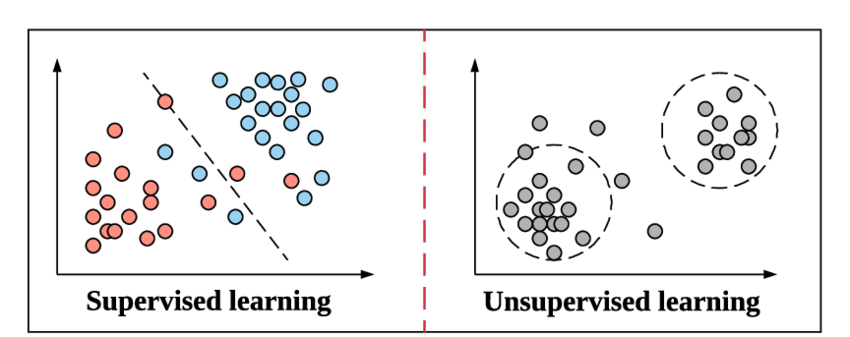
\includegraphics[width=12cm, keepaspectratio]{fig/cap1/Examples-of-Supervised-Learning-Linear-Regression-and-Unsupervised-Learning.png}
	\caption{Diferența dintre modul de funcționare al învățării supervizare și învățării nesupervizate \cite{fig:sup_and_unsup}}
	\label{fig:sup_and_unsup_learning}
\end{figure}

\subsection*{Învățarea cu întărire}
Învățarea cu întărire este o metodă de învățare prin interacțiuni repetate a unui \textit{agent (software agent)} cu mediul, cu urmărirea atingerii unui anumit scop (\autoref*{fig:reinf_learning}). Interacțiunile se bazează pe acțiunile luate de agent la stimulii mediului, pentru care v-a primit o recompensă de la acesta în funcție de beneficiul adus îndeplinirii scopului. Recompensele primite au rolul de a îmbunătății capacitatea agentului de a lua cea mai bună decizie din starea în care acesta se afla la momentul acțiunii. Scopul pe termen lung al agentului este maximizarea numărului de recompense primite. După repetate interacțiuni cu mediul, capacitatea agentului de a lua decizii bune se v-a crește, iar drumul acestuia prin mediu va tinde spre optim.
\begin{figure}[h]
	\center
	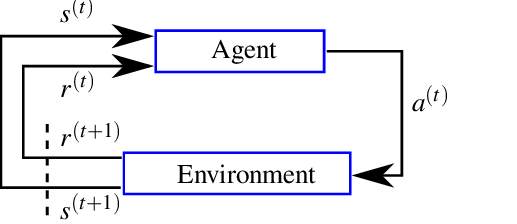
\includegraphics[width=11cm, keepaspectratio]{fig/cap1/The-reinforcement-learning-paradigm-consists-of-an-agent-interacting-with-an.png}
	\caption{Modul de funcționare al învățării cu întărire \cite{fig:reinforcement}}
	\label{fig:reinf_learning}
\end{figure}

\subsection*{Obiective}
Această lucrare își propune folosirea rețelelor convoluționale pentru clasificarea a trei clase/stării mentale diferite. Metoda de clasificare se bazează pe reprezentarea informațiilor statistice și spectrale a undelor cerebrale sub forma unor imagini alb-negru. Datele EEG \textit{(Electroencefalograma)} au fost extrase cu ajutorul caștii valabile comercial, Muse 2016. Datele extrase au fost prelucrate și etichetate, rezultând 414 atribute și clasa de care aparțin, neutru, relaxat sau concentrat. După extragerea atributelor, au fost selectate și normalizate în intervalul [0:1] 400 de atribute pentru a putea reprezenta o imagine alb-negru de dimensiunea 20x20. După antrenarea clasificatorului cu aceste imagini, acuratețea acestuia la prezicerea imaginilor care nu se aflau in setul de date de antrenare, a fost de 90\%.

\section{Soluții existente}
Apariția unor soluții comerciale \textit{low-cost} non-invazive a facut posibilă înregistrarea și analiza undele cerebrale în afara domeniului medical \cite{online:emotiv}. În principal, aceste dispozitive sunt folosite în activități simple de interfațare a creierului cu calculatorul \textit{(BCI - Brain-Computer Interface)}. Raportul zgomot-semnal util mare și eșantionarea imperfectă reprezentând dezavantajele acestor aparate comparativ cu cele de nivel medical. Acest lucru însă nu a împiedicat apariția a tot mai multor studii care folosesc aceste aparate ca o resursă \cite{consumer-eeg:2018}.



EEG\cite{eeg:2018}

EEG-CNN\cite{eeg-cnn:2020}

\textbf{TODO\_PLACEHOLDER}
\begin{itemize}
	\item Utilizare casca pt clasificare EEG de detectare a starii
	\subitem Scriu despre articolul de clasificare EEG de la cei care au scris articolul cu CNN
	\subitem O sa scriu despre articolul cu CNN
\end{itemize}
\section{Structurare pe capitole}
Lucrarea este structurată după cum urmează. \textit{\autoref{ch:2studiu_teoretic}} prezintă o introducere a ceea ce înseamna și modul în care funcționează rețelele neuronale de tipul \textit{feedforward} ca mai apoi să poată fii folosite ca suport în înțelegerea funcționalității rețelelor convoluționale. V-or fii menționate avantajele și prezentate aplicațiile de succes ale acestora. Tot aici, v-or fii prezentate bazele undelor cerebrale, ce sunt acestea, cum funcționează și felul în care pot fii detectate. În \textit{\autoref{ch:3implementare}} este prezentat modul de implementare al soluției împreună cu detaliile tehnice aferente. Explicarea tehnicilor de extragere și prelucrare a datelor, detalii privind arhitectura rețelei folosite și rezultatele produse de aceasta se v-or regăsi la finalul acestui capitol. Finalul lucrării conține \textit{\autoref{ch:4concluzii}}, care aduce concluzii legate de tema acestei lucrări.
%!TEX root = ./main.tex
\chapter{Studiul teoretic. Tehnologii folosite}\label{ch:2studiu_teoretic}
\textbf{TODO} Adauga referintele bibliografice aici, intr-un paragraf \cite{neuralnetbook:2015}

Acest capitol are rolul de a prezenta noțiuni și aspecte fundamentale legate de rețelele convoluționale și undele cerebrale, elemente de bază ale acestei lucrări. În prezentarea rețelelor convoluționale se va porni de la perceptronul simplu, care constituie fundamentul acestor algoritmi, apoi va fi prezentată o rețea alcătuită din perceptroni, iar la final va fi prezentată rețeaua convoluțională, construită cu ajutorul noțiunilor și elementelor provenite de la rețeaua neuronală. Undele cerebrale, ce sunt acestea, cum se formează și ce reprezintă va fi prezentat spre finalul acestui capitol.

\section{Rețele neuronale}
Rețelele neuronale artificiale reprezintă un sistem de calcul inspirat după modelul rețelelor neuronale biologice, atât ca și structură, cât și ca mod de procesare a informației. Neuronul artificial reprezintă unitatea elementară a unei rețele neuronale artificiale. Precum neuronul biologic, care conține dendrite și axioni, neuronul artificial imită această structură prin noduri de intrare si noduri de ieșire.
\subsection{Perceptronul}
Conceptele fundamentale ale neuronului artificial provin din modelul perceptronului introdus de către \textit{Frank Rosenblatt (1958)} \cite{rosenblatt1962principles} pe baza cercetărilor anterioare ale lui \textit{Warren McCulloch} și \textit{Walter Pitts} \cite{McCulloch:427611}.

Perceptronul primește o serie de valori la intrare, $x_1, x_2, x_3\dots$, și produce o singură ieșire. Pentru calculul ieșirii, sunt folosite așa numitele \textit{ponderi (weights)}, notate cu $w_1, w_2, w_3,\dots$, numere reale reprezentând importanța fiecărei intrări în determinarea ieșirii.
\begin{figure}[ht]
\centering
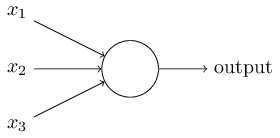
\includegraphics[width=10cm, keepaspectratio]{fig/cap2/perceptron.png}
\caption{Reprezentarea grafică a unui perceptron}
\end{figure}

Astfel, ieșirea perceptronului, este determinată de suma ponderată $\sum_i x_iw_i$ comparată cu o valoare reală numită \textit{prag}. Această comparație reprezintă o funcție pentru determinarea ieșirii $y$, denumită \textit{funcție de activare}. Matematic, funcția de activare a perceptronului este reprezentată de o formă discretă a funcției \textit{treaptă unitate}, descrisă de ecuația \eqref{eq:perceptron-simplu}.
\begin{equation}
y = 
	\begin{dcases}
	0 & : \sum_i x_iw_i \le prag\\
	1 & : \sum_i x_iw_i > prag
	\end{dcases}
\label{eq:perceptron-simplu}
\end{equation}

Putem simplifica modul prin care perceptronii sunt descriși, rescriind $\sum\nolimits_i x_iw_i$ ca fiind produsul cartezian $x \cdot w$, unde $x$ și $w$ sunt vectori care conțin intrările $x_i$ respectiv ponderile $w_i$. A doua modificare pe care o putem face este să mutăm termenul $prag$ în partea stângă a inegalității, denumindu-l \textit{bias/offset}, $b=-prag$. Astfel, ecuația \eqref{eq:perceptron-simplu} devine:
\begin{equation}
y = 
	\begin{dcases}
	0 & : x \cdot w + b \le 0\\
	1 & : x \cdot w + b > 0
	\end{dcases}
\label{eq:perceptron}
\end{equation}

Bias-ul poate fii considerat ca o intrare suplimentară de valoate $x_0 = 1 \text{ și } w_0 = b$ care permite translatarea funcției de activare la stânga sau la dreapta.

\subsection{Perceptronul multistrat}\label{subch:mlp}
Prin conectarea mai multor perceptroni rezultă rețeaua numită „perceptronul multistrat” \textit{(Multi-layer Perceptron - MLP)}. Aceasta este formată dintr-o succesiune de perceptroni complet conectați, așezați înntr-un stratz de intrare, unul sau mai multe straturi ascunse \textit{(hidden layer)} și un strat de ieșire. Ieșirile unui strat reprezintă intrările pentru stratul următor. Rețeaua care conține mai multe straturi ascunse poartă denumirea de \textit{„rețea neuronală adâncă” ("deep neural network")}, iar în cazul în care aceasta conține un singur strat ascuns poartă denumirea de \textit{„rețea neuronală superficială” ("shallow neural network")}. \autoref{fig:mlp} prezintă o astfel de rețea.

\begin{figure}[h]
\center
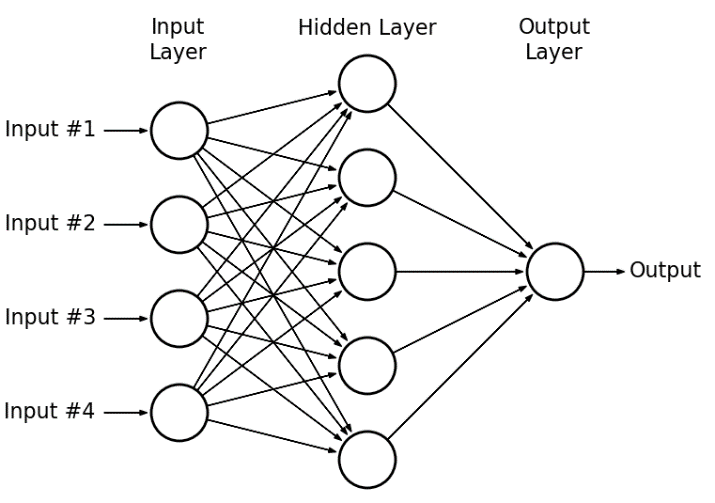
\includegraphics[width=\textwidth, keepaspectratio]{fig/cap2/mlp.png}
\caption{Rețea de tipul perceptron multistrat}
\label{fig:mlp}
\end{figure}

Rețeaua prezentată mai sus este de tip \textit{propagare înainte (feed-forward)}, adică, informația în rețea circulă într-o singură direcție, de la stânga la dreapta. Rezultatul procesării informațiilor de către primul strat de neuroni va reprezenta intrarea pentru stratul al doilea, astfel ieșirile acestuia având o semnificație mai abstractă și complexă comparativ cu primul strat. Cu fiecare strat ascuns adăugat rețelei, nivelul de abstractizare al informației va crește, astfel deciziile luate de rețea devenind tot mai sofisticate.

Limitarea acestui tip de rețea poate fii observată încercând să aplicăm schimbări mici ponderilor $w$ conexiunilor (sau a $bias$-ului) unui strat pentru a obține o schimbare mică a ieșirii rețelei. Analitic, acest lucru se rezumă la următoarea ecuație:
\begin{equation}
\Delta y\approx\sum_i\frac{\partial y}{\partial w_i}\Delta w_i + \frac{\partial y}{\partial b}\Delta b
\end{equation}
În realitate însă acest lucru nu se întâmplă întotdeauna. Aceste mici modificări pot determina schimbarea complet a stării\footnote{Acest lucru poate fi observat în graficul funcției de activare al perceptronului din \autoref{fig:sig+step+tanh+relu}}, spre exemplu de la 1 la 0. Acest comportament poate declanșa o schimbare foarte complicată și greu de controlat în întreaga rețea.

Limitarea dată de capacitatea perceptronului de clasificare binară, poate fii rezolvată însă folosind un alt tip de funcție de activare. 

\subsection{Neuronul}\label{subch:neuronul}
Neuronul artificial este foarte asemănător cu perceptronul prezentat anterior. Acesta este format dintr-un vector de intrări $x$, un vector al ponderilor $w$, un bias $b$ și o ieșire $y$. Valorile vectorului de intrare $x$ nu sunt însă limitate la valorile 1 sau 0, neuronul sigmoid fiind capabil să proceseze valori reale. Precum $x$, ieșirea $y$ a neuronului poate lua valori reale. \autoref{fig:neuron} prezintă un astfel de neuron.
\begin{figure}[ht]
\centering
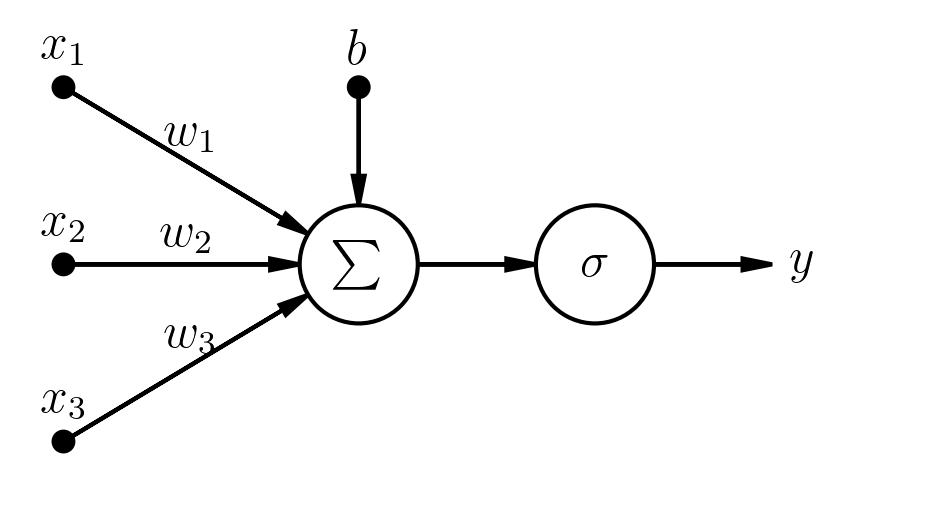
\includegraphics[width=10cm,keepaspectratio]{fig/cap2/artificial-neuron.png}
\caption{Reprezentarea grafică a unui neuron sigmoid}\label{fig:neuron}
\end{figure}

Neuronul care folosește \textit{funcția sigmoid} ca și funcție de activare, dată de ecuația \eqref{eq:sigm}, se numește neuron sigmoid și este cel mai simplu tip de neuron artificial datorită proprietăților funcției logistice la derivare\footnote{Derivabilitatea funcțiilor de activare este o cerință în cadrul folosirii algoritmului de antrenare prin back-propagation prezentat în \S\ref{subch:antrenare}}.

\begin{equation}
\sigma(z) = \frac{1}{1+e^{-z}} \quad,\text{unde }z= w\cdot x + b
\label{eq:sigm}
\end{equation}

Analizând graficele din \autoref{fig:sig+step+tanh+relu} putem observa faptul că funcția sigmoid este de fapt o versiune netezită a funcției treaptă unitate. Acest lucru ne asigură că schimbările mici efectuate atât în vectorul ponderilor $w$ cât și în $b$ vor fi reflectate în ieșire și că nu vom avea salturi bruște de la 0 la 1 la ieșirea neuronului.
Totuși, modelul perceptronului poate fii simulat folosind funcția sigmoid. Atunci când $z\rightarrow\infty$, $\sigma(z)\approx 1$, iar când $z\rightarrow-\infty$, $\sigma(z)\approx 0$. Folosind astfel de funcții de activare ne ajută să găsim ponderile potrivite mult mai ușor și putem afla felul în care modificările acestora afectează ieșirea.

În general, se folosesc funcții derivabile pe întreg domeniul de definiție, care nu au treceri bruște de la un capăt la altul, pentru a facilita antrenarea rețelei. În practică se mai folosesc funcții precum \textit{tangenta hiperbolică}:
\begin{equation}
\tanh(z)=\frac{e^z - e^{-z}}{e^z + e^{-z}}
\end{equation}
sau \textit{funcția unitate liniară rectificată (ReLU)}:
\begin{equation}
R(z)=\max(0,z)
\label{eq:relu}
\end{equation}

\autoref{fig:sig+step+tanh+relu} prezintă graficele diferitor funcții de activare.
\begin{figure}[ht]
\centering
\subfloat[Funcția sigmoid]{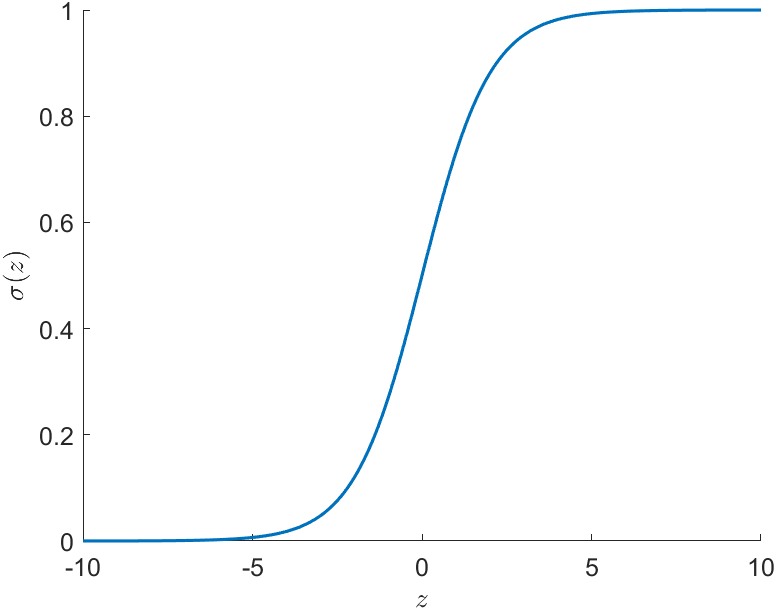
\includegraphics[width=6.9cm, keepaspectratio]{fig/cap2/sig.png}\label{fig:sigmoid}}
\qquad
\subfloat[Funcția treaptă unitate]{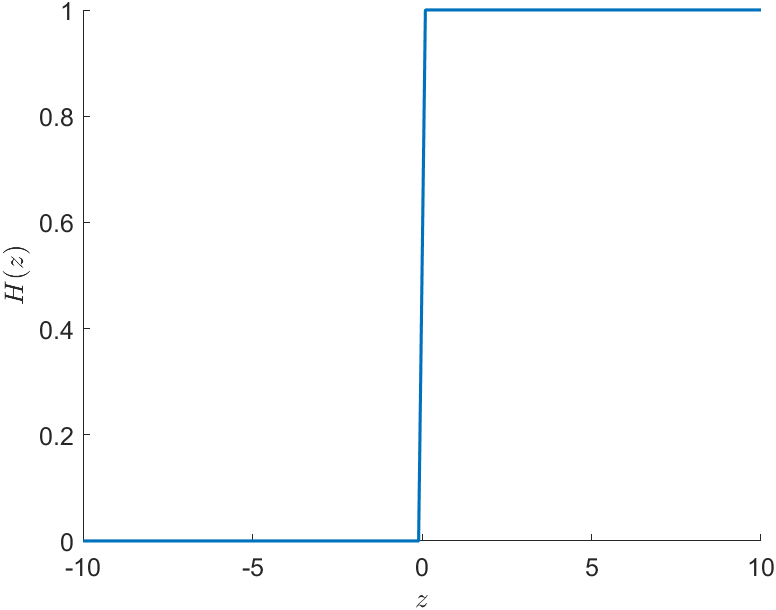
\includegraphics[width=6.9cm, keepaspectratio]{fig/cap2/step.png}\label{fig:step}}
\qquad
\subfloat[Funcția tangenta hiperbolică]{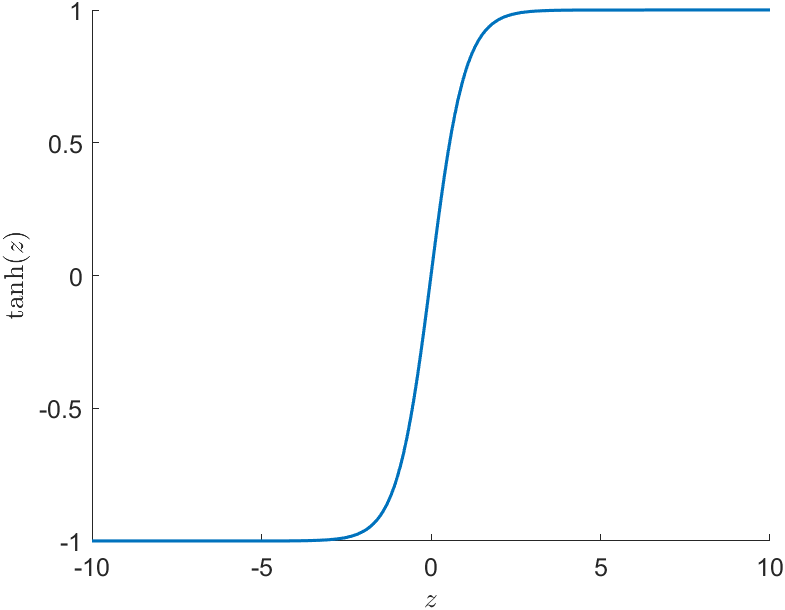
\includegraphics[width=6.9cm, keepaspectratio]{fig/cap2/tanh.png}\label{fig:tanh}}
\qquad
\subfloat[Funcția unitate liniară rectificată]{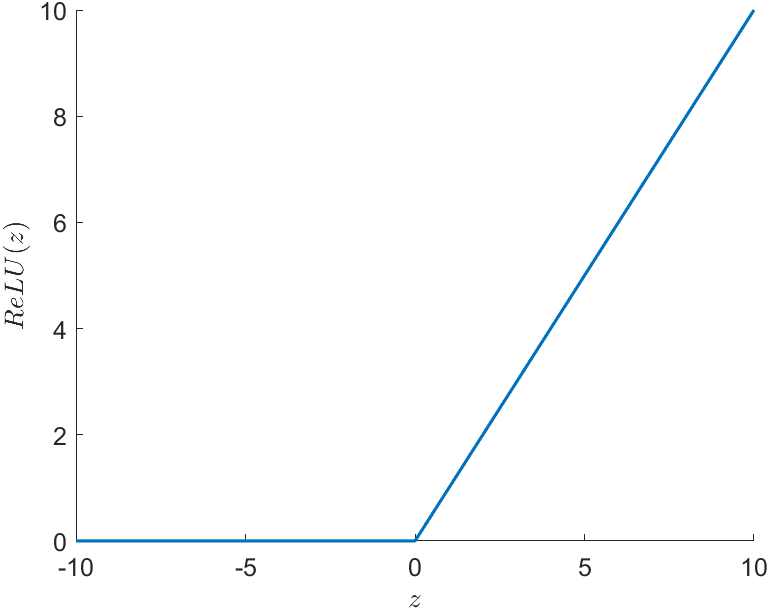
\includegraphics[width=6.9cm, keepaspectratio]{fig/cap2/relu.png}\label{fig:relu}}
\caption{Funcții de activare}\label{fig:sig+step+tanh+relu}
\end{figure}

Este necesar de menționat faptul că aceste funcții se folosesc în special pentru neuronii aflați în straturile ascunse ale rețelei, stratul de ieșire folosind de obicei funcții logistice pentru clasificări binare și funcția \textit{softmax} pentru clasificări multi-clasă.

\subsection{Antrenarea rețelelor}\label{subch:antrenare}
Algoritmul prin care se realizează antrenarea rețelelor de tipul feedforward, poartă denumirea de \textit{algoritm de propagare înapoi (back-propagation)}. Acest algoritm a fost făcut faimos de către David Rumelhart, Geoffrey Hinton, și Ronald Williams în 1986 \cite{rumelhart1986}. Algoritmul constă în modificarea repetată a ponderilor conexiunilor din rețea în încercarea de a minimiza o funcție care reprezintă eroarea dintre rezultatul așteptat și cel obținut. Funcțiile folosite cu scopul de a fii minimizate se numesc \textit{funcții obiectiv} sau \textit{funcții de cost} (\S\ref{subch:f-cost}).

\subsubsection*{Ecuațiile algoritmului back-propagation}
Algoritmul clasic de back-propagation a fost inițial conceput să rezolve probleme de regresie folosind funcții de activare sigmoide. Totuși, acesta poate fii aplicat și problemelor de clasificare cu sau fară astfel de funcții de activare. Pentru a putea face o descriere matematică asupra modului de funcționare al algoritmului, este necesară folosirea următoarelor notații \cite{neuralnetbook:2015}:
\begin{enumerate}
\item $C$ pentru a reprezenta o funcție de cost
\item $w_{jk}^l$ pentru specificarea ponderii conexiunii de la neuronul $k$ în stratul $l-1$ către neuronul $j$ în stratul $l$.
\item $b_j^l$ pentru bias-ul neuronului $j$ din stratul $l$
\item $a_j^l$ pentru activarea neuronului $j$ din stratul $l$
\end{enumerate}
$a_j^l$ depinde de activarea neuronului din stratul $l-1$ conform ecuației
\begin{equation}
a_j^l=\sigma(\sum_k w_{jk}^l a_k^{l-1} + b_j^l)
\end{equation}
unde $k$ reprezintă toți neuronii din stratul $l-1$. Folosind aceste notații pot fii descrise cele patru ecuații fundamentale ale acestui algoritm:
\begin{enumerate}
\item Ecuația pentru determinarea erorii din stratul de ieșire $L$
\begin{equation}
\delta_j^L=\frac{\partial C}{\partial a_j^L}\sigma'(z_j^L)
\label{eq:out-err}
\end{equation}
\item Ecuație pentru determinarea erorii din stratul $l$ în raport cu eroarea din stratul $l+1$
\begin{equation}
\delta^l = ((w^{l+1})^T \delta^{l+1}) \odot \sigma'(z^l)
\label{eq:back-prop-err}
\end{equation}
\item Ecuație pentru determinarea ratei de schimbare a funcției de cost în funcție de orice bias din rețea
\begin{equation}
\frac{\partial C}{\partial b^l_j} = \delta^l_j
\label{eq:cost-w}
\end{equation}
\item Ecuație pentru determinarea ratei de schimbare a funcției de cost în funcție de orice pondere din rețea
\begin{equation}
\frac{\partial C}{\partial w^l_{jk}} = a^{l-1}_k \delta^l_j
\label{eq:cost-b}
\end{equation}
\end{enumerate}

\subsubsection*{Aplicarea algoritmului back-propagation}
Inițial toți parametrii rețelei (ponderile $w$ și bias-ul $b$) vor fii inițializați aleator\footnote{Nu este neapărat ca parametrii rețelei să fie inițializați aleator, existând mai multe metode de inițializare}. Urmează apoi etapa de propagarea înainte a datelor din setul de date de antrenare și a comparării rezultatului prezis în comparație cu cel real. Această eroare se calculează conform ecuației \eqref{eq:out-err}, iar mai apoi va fii propagată înapoi în rețea, strat cu strat, începând cu stratul $l = L-1$, conform ecuației \eqref{eq:back-prop-err}. Parametrii vor fi ajustați în funcție de gradientul funcției de cost conform ecuațiilor \eqref{eq:cost-w} și \eqref{eq:cost-b}. Gradientul funcției de cost se calculează folosind un algoritm de optimizare, cel mai folosit algoritm împreună cu back-propagation este metoda gradientului \textit{(gradient descent)}. Algoritmul se repetă pentru un numar stabilit de pași (aleși experimentali) sau până când eroarea $\delta^L$ scade sub o valoare impusă. Odată cu finalizarea algoritmului, rețeaua va fii pregătită să proceseze date pe care nu le-a întâlnit în setul folosit la antrenare și să facă predicții asupra acestora.
\begin{figure}[ht]
\centering
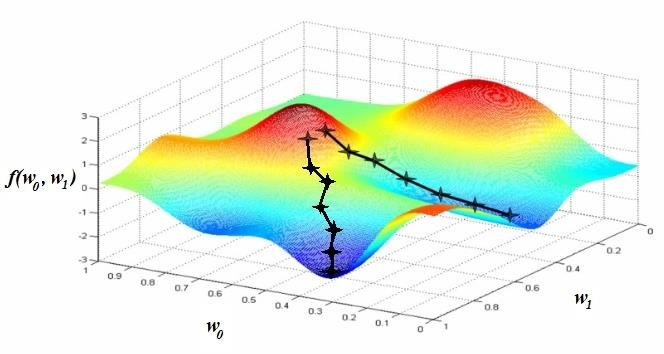
\includegraphics[width=12cm, keepaspectratio]{fig/cap2/grad-desc.jpg}
\caption{Ilustrarea algoritmului de optimizare gradient descent folosit în back-propagation\cite{vrejoiu:2019}}
\end{figure}

\subsection{Funcții de cost}\label{subch:f-cost}
O funcție de cost este o funcție de forma \cite{neuralnetbook:2015}
\begin{equation}
C(w,b,S^T,E^T)
\label{eq:cost-form}
\end{equation}
unde $w$ și $b$ reprezintă parametrii rețelei $S^T$ intrarea unui eșantion de date de antrenare și $E^T$ ieșirea dorită din eșantionul respectiv.

Rezultatul dat de asemenea funcții este un număr care reprezintă performanța rețelei de a face preziceri pe baza modificărilor aduse parametrilor acesteia. Se urmărește prin diferite \textit{tehnici de optimizare} minimizarea acestei funcții, valoarea returnată purtând denumirea de \textit{eroare/cost/loss}. În anumite situații însă, spre exemplu în cazul învățării cu întărire, scopul este de a maximiza această funcție, rezultatul fiind denumit \textit{recompensă}.

Atât funcțiile de cost, cât și tehnicile de optimizare ale acestora trebuie alese în funcție de problema în cauză, neexistând o soluție universal valabilă. Empiric, funcțiile de cost se pot împărți în două categorii:
\begin{itemize}
\item \textbf{pentru probleme de regresie}: eroarea medie absolută \textit{(L1 loss)}, eroarea medie pătratică \textit{(L2 loss)},  Huber Loss
\item \textbf{pentru problemele de clasificare}: funcția de cost logaritmică \textit{(cross-entropy)}, categorical cross-entropy, divergența Kullback–Leibler
\end{itemize}

\section{Rețele convoluționale}
Rețelele convoluționale sunt un tip specific de rețele neuronale adândci inspirate din modul de reconoaștere al tiparelor în cortexul vizual uman. Arhitectura acestor rețele s-a dovedit a fi foarte eficientă atât în clasificarea imaginilor cât și în timpul necesar antrenării acesteia.

Una din primele rețele convoluționale de succes a fost \textit{LeNet5 (1989)} \cite{LeNet5}, după repetate iterații începând cu anul 1988. Această rețea a fost folosită în principal pentru detectarea cifrelor și codurilor poștale.

În ziua de astăzi rețelele neuronale convoluționale sunt folosite în diverse aplicații, predominant fiind cele pe baza analizei imaginilor, precum detectarea și recunoașterea obiectelor din seturi de date cu mii de categorii, de exemplu \textit{VGGNet} \cite{simonyan2014deep} pe setul de date \textit{ImageNet}, determinarea profunzimii scenelor din imaginile video 2D \cite{zhou2017unsupervised}, practic imitând principiul \textit{LIDAR}\footnote{Light Detection And Ranging - reprezintă un sistem similar de funcționare cu radar-ul, care utilizează laser-ul pentru a afla distanța până la țintă}, segmentarea obiectelor din scenă \textit{(semantic segmentation)}. Rețelele convoluționale și-au găsit folosința și în aplicații care nu implică în mod direct imagini, cum ar fii procesarea limbajului natural sau clasificarea evenimentelor audio \cite{cnnaudioclass}.

\subsection*{Arhitectura}
Structura unei rețele convoluționale este formată din două părți.
Partea convoluțională, compusă din stratul de convoluție cu funcția de activare aplicată ieșirii acestuia și stratul de reducere a dimensionalității. A doua parte a structurii este partea de clasificare alcătuită din straturi de neuroni complet conectați asemenea rețelei MLP prezentate în \S\ref{subch:mlp}. \autoref{fig:cnn-arch} prezintă o astfel de arhitectură.
\begin{figure}[ht]
\centering
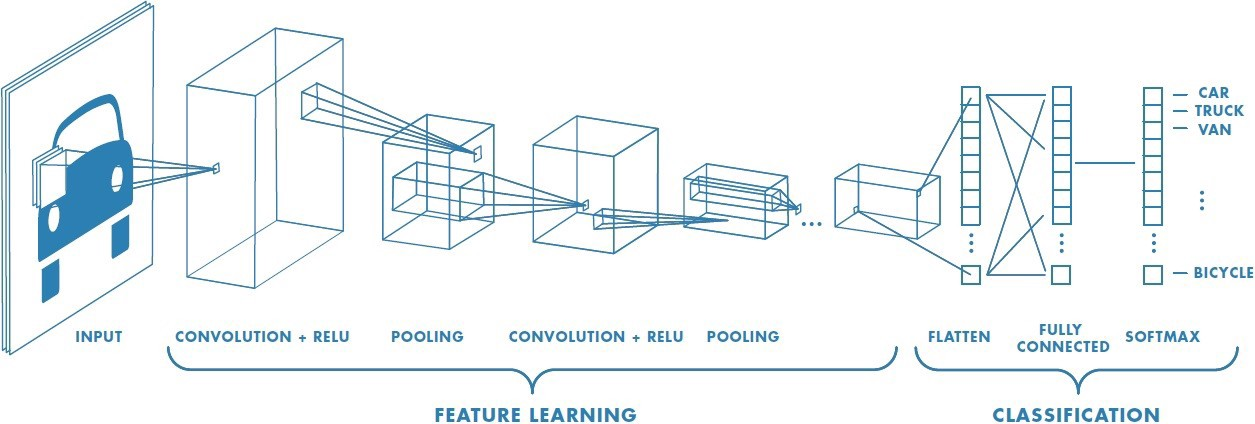
\includegraphics[width=\textwidth]{fig/cap2/cnn-arch.jpeg}
\caption{Arhitectura generală a unei rețele convoluționale}
\label{fig:cnn-arch}
\end{figure}

\subsection*{Straturile de convoluție}
Rețelele convoluționale sunt denumite după operația centrală acestora, operația de convoluție. Matematic, operația de convoluție reprezintă rezultatul combinării a două funcții pentru a forma o a treia. Această operație poate fi descrisă în varianta discretă în spațiul 2D sub următoarea formă
\begin{equation}
(f*g)[i,j]=\sum\sum f[m,n]g[i-m,j-n]
\label{eq:conv-dis-2D}
\end{equation}

În straturile convoluționale, spre deosebire de cele complet conectate, neuronii ascunși din stratul $l$ sunt conectați la un grup localizat de neuroni din stratul $l-1$ denumit câmp receptor \textit{(receptive field)}. Câmpul receptor reprezintă zona în care este aplicat filtrul/nucleul de convoluție asupra matricei de intrare. Crearea stratului $l$ de neuroni ascunși se realizează aplicând un filtru/nucleu de convoluție de dimensiune $H\times W$, care va fi mutat peste întreaga imagine de intrare pornind din colțul stânga sus și deplasându-se pe orizontală și pe verticală cu un anumit „pas” \textit{(stride)} notat $s$. În exemplul din \autoref{fig:mat-conv} pasul folosit este de $s=1$. Se poate observa faptul că odată cu aplicarea operației de convoluție rezultă o reducere a dimensionalității a matricei rezultate. Acest lucru poate fi remediat brodând cu zero-uri \textit{(zero padding)} marginile matricei de intrare.
\begin{figure}[ht]
\centering
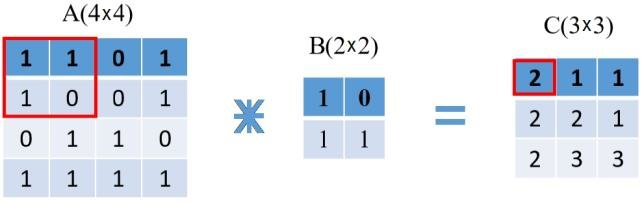
\includegraphics[width=10cm, keepaspectratio]{fig/cap2/conv-op.jpg}
\caption{Exemplificarea convoluției a două matrici \cite{vrejoiu:2019}}
\label{fig:mat-conv}
\end{figure}

Asupra rezultatului de  convoluție dintre filtru și matricea de intrare se aplică o funcție de activare, care este adesea de tip ReLU, amintită în \S\ref{subch:neuronul}. Matricea rezultată în urmă operației de convoluție și aplicarea funcției de activare poartă denumirea de hartă de caracteristici \textit{(feature map)} sau hartă de activare \textit{(activation map)}.

Un strat de convoluție este alcătuit dintr-o sumedenie de hărți de caracteristici create folosind diferite tipuri de filtre. Fiecare strat adăugat rețelei, va crea hărți care vor captura caracteristici tot mai complexe din imaginea inițială.
\begin{figure}[ht]
\centering
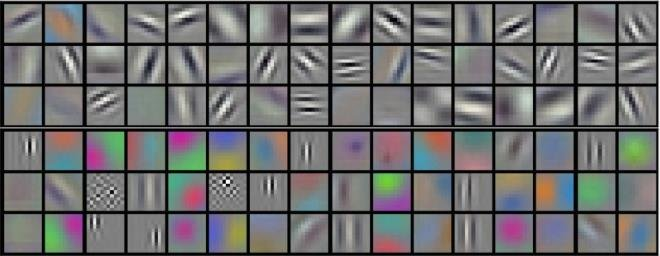
\includegraphics[width=10cm, keepaspectratio]{fig/cap2/alexnet-filters.jpg}
\caption{Filtrele învățate în primul strat de convoluție de către rețeaua AlexNet \cite{alexnet:2012}}
\label{fig:alexnet-filters}
\end{figure}

\subsection*{Reducerea dimensionalității}
Deseori, după stratul de convoluție este aplicat un strat de reducere a dimensionalității \textit{(pooling)}, cunoscut și sub numele de subeșantionare. Acesta are rolul de a micșora dimensiunile spațiale ale hărților de caracteristici și de a reduce numărul de parametrii antrenabili, dar în același timp de a păstra informațiile esențiale. Tehnicile folosite uzual pentru operația de \textit{pooling} sunt \textit{Average Pooling, Max Pooling, Sum Poolling}. Aceste tehnici au la bază folosirea unei ferestre de dimensiuni relativ mici (de obicei $2\times2$), din care vor fi extrase valorile maxime în cazul Max Pooling, valorile medii pentru Average Pooling și suma tuturor valorilor pentru Sum Pooling. Empiric s-a observat faptul ca de cele mai multe ori tehnica Max Pooling are cele mai bune rezultate. \autoref{fig:maxpooling} exemplifică aplicarea acestei tehnici.
\begin{figure}[ht]
\centering
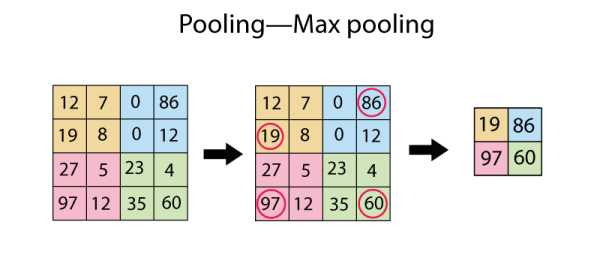
\includegraphics[width=\textwidth, keepaspectratio]{fig/cap2/poolingmax.png}
\caption{Exemplificarea aplicării tehnicii Max Pooling \cite{online:pooling}}
\label{fig:maxpooling}
\end{figure}

Operațiile de pooling descrise anterior pot fi înlocuite folosind în stratul convoluțional un pas de deplasare al filtrelor mai mare ca 1 sau folosind un strat convoluțional special cu dimensiunea filtrului $1\times1$ și cu pasul $s>1$. Această operație poate fi benefică din punct de vedere computațional, deoarece atât operația de convoluție cât și operația de subeșantionare sunt aplicate în același timp însă poate crește dificultatea de antrenare a rețelei datorită creșterii numărului de parametrii antrenabili introduși în rețea comparativ cu tehnicile de pooling care nu conțin nici un parametru, sunt operații fixe.

Subeșantionarea folosind operațiile de pooling clasice poate cauza probleme rețelelor convoluționale prin pierderea informației poziționale ale diferitelor obiecte prezente în imagine. Scopul inițial al introducerii acestui strat a fost de a reduce numărul de parametrii ai rețelei, deci reducerea timpului de antrenare a rețelei. Avansuri în dispozitive hardware tot mai puternice a redus nevoia unei astfel de tehnici, astăzi multe arhitecturi înlocuind această metodă de reducere a dimensionalității cu straturi speciale de convoluție precum \textit{Separable Convolutions} și \textit{Dilated Convolutions}.

\subsection*{Stratul complet conectat}
Pentru a putea face legătura între straturile convoluționale și clasificatorul final, ieșirea din straturile convoluționale trebuie transformată din dimensiunea $H\times W\times D$, într-un vector coloană $H\times1$. Această operație poartă denumirea de \textit{aplatizare (flatten)} și este inclusă intr-un strat separat denumit \textit{strat de aplatizare (flatten layer)}.

Odată transformată ieșirea sub formă de vector, aceasta este folosită ca intrare, de obicei, pentru rețele neuronale multistrat. Această rețea folosește pe stratul de ieșire funcția de activare \textit{softmax}, care are rolul de a furniza un vector de probabilități cu dimensiunea egală cu numărul claselor, fiecare poziție a vectorului reprezentând o probabilitate pentru clasa aferentă.

Se mai pot folosi în schimbul rețelelor neuronale și alte tehnici de clasificare, precum \textit{mașini cu vectori suport (SVM)}.

\section{Undele cerebrale}
Creierul uman conține miliarde de celule specifice sistemului nervos, înalt specializate, numite \textit{neuroni}, cu capacitatea de a genera, transmite și recepționa semnale electro-chimice. Un neuron este alcătuit din \textit{corp celular}, \textit{dendrite} și \textit{axon} (Fig. \ref{fig:neuron-anatomy}). Legătura dintre mai mulți neuroni se numește \textit{sinapsă} și este realizată între axonul neuronului presinaptic și dendritele sau corpul celular neuronului postsinaptic. În creierul uman, un neuron formează, în medie, aproximativ 7000 de conexiuni sinaptice. Fiecare neuron deține o diferență de potențial în jurul membranei sale numită \textit{potențial local}. În momentul în care tensiunea electrică crește brusc, neuronul generează un puls electro-chimic denumit \textit{potențial de acțiune}, care străbate rapid axonul neuronului activând conexiunile sinaptice ale acestuia.
\begin{figure}[ht]
\centering
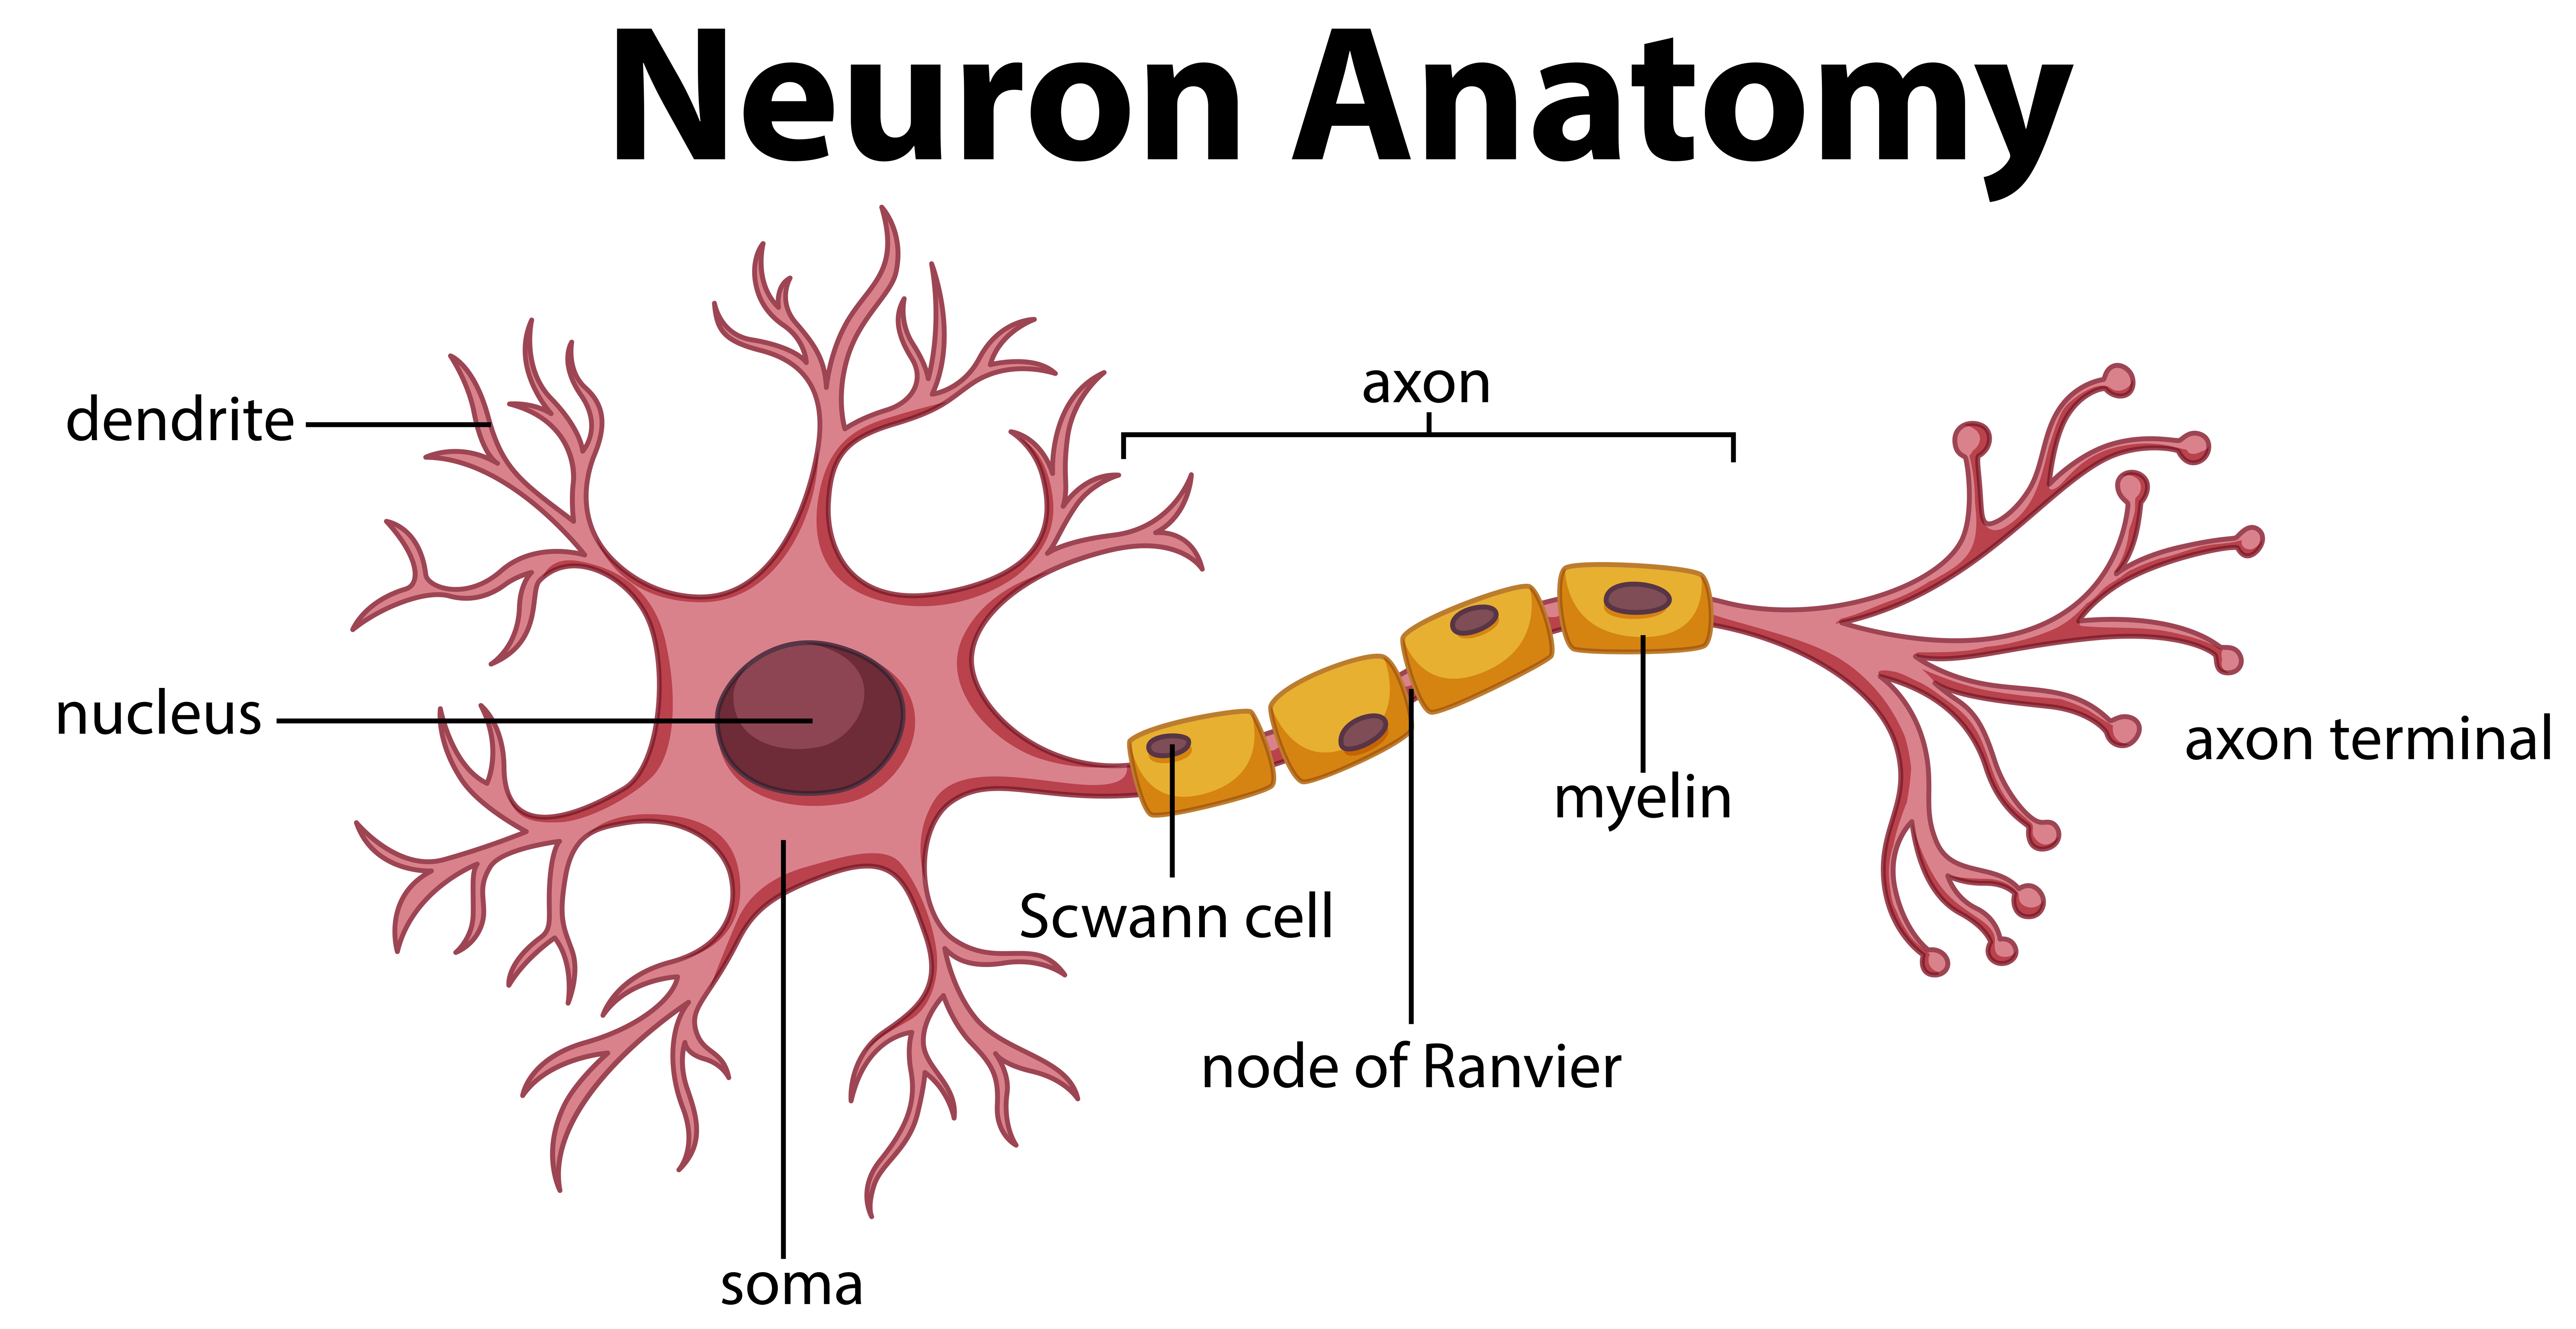
\includegraphics[width=\textwidth, keepaspectratio]{fig/cap2/neuron-anatomy.jpg}
\caption{Anatomia unui neuron tipic \cite{online:neuron-anatomy}}
\label{fig:neuron-anatomy}
\end{figure}

Descărcările electrice repetate și sincronizate ale neuronilor rezultă în așa numitele \textit{unde cerebrale}, cu benzile de frecvență cuprinse între 0.5 - 50 \si{\hertz}. \textit{Electroencefalografia (EEG)} este tehnica de detectate și înregistrate în timp a activității cerebrale. Aceasta poate fi folosită în două moduri, invaziv sau neinvaziv. 

Electroencalografia invazivă presupun așezarea electrozilor direct pe suprafața creierului. Folosirea acestei metode de înregistrare a undelor cerebrale rezultă în date achiziționate fără zgomot și precise referitor la zona creierului studiată. Dezavantajul este însă marcat de complexitatea metodei, necesitând intervenție chirurgicală cu riscuri mari.

Achiziția undelor cerebrale într-un mod neinvaziv constă în plasarea electrozilor pe scalp, astfel fiind eliminată necesitatea unei operații și a complexității procedurii. Folosind această metodă datele achiziționate vor fi alterate de zgomot produs de contracțiile mușchilor din zona capului, datele având nevoie de preprocesare înainte de a putea fi folosite.

Există cinci tipuri de bază de unde cerebrale, fiecăreia fiindui atribuită o literă grecească, după cum urmează \textit{delta, teta, alfa, beta, gama}. Undele cerebrale se modifică în funcție de activitatea desfășurată și de dispoziție. Însemnătatea acestora este corelată cu locația detectării în creier.

\subsubsection*{Delta}\label{ssch:delta}
Undele delta au cea mai scăzută bandă de frecvența dintre toate undele cerebrale, încadrându-se în intervalul 0.5-4 \si{\hertz}. Se întâlnesc cel mai des în timpul unui somn adânc sau în timpul meditației profunde. Această stare mentală stimulează regenerarea și vindecarea corpului.

\subsubsection*{Teta}\label{sush:teta}
Banda de frecvență caracteristică undelor teta e între 5 și 8 \si{\hertz}. Adesea, acestea sunt foarte ușor detectabile în momentele în care visăm. Starea mentală teta mai poate fi observată și în momentul unor activități foarte comune, în care procesul de realizare devine automat. Această stare dă naștere unui șir de gândire și idei liber în care creativitatea este sporită.

\subsubsection*{Alfa}\label{sush:alfa}
Undele alfa, cu banda de frecvență între 9 și 14 \si{\hertz},  reprezintă starea de relaxare conștientă. Plimbările prin parc, momentele de relaxare după îndeplinirea unei sarcini, reflecția  sau meditația ușoară reprezintă momente în care undele alfa sunt proeminente.

\subsubsection*{Beta}\label{sush:beta}
Undele beta, având banda de frecvență între 15 și 40 \si{\hertz}, sunt asociate cu activitatea mentală normală. Acestea sunt prezente în momente precum concentrarea asupra unei probleme, învățarea de noi concepte, stare de alertă sau luarea deciziilor. Concret, această stare este caracteristică gândirii active.

\subsubsection*{Gama}\label{sush:gama}
Undele gama au banda de frecvență cea mai înaltă, >40 \si{\hertz}, fiind asociate cu procesarea simultană a informațiilor din zone diferite ale creierului. Acestea au fost inițial încadrate ca fiind „zgomot cerebral” până când cercetătorii au observat o activitate accentuată a acestora în stări cognitive și concentrație intensă. Modul de generare al acestor unde cerebrale este încă necunoscut, frecvența acestora fiind peste capacitatea de descărcare a neuronilor. 

%!TEX spellcheck=ro_RO
%!TEX root = ./main.tex
\chapter{Prezentarea aplicației}\label{ch:3implementare}
\section{Etape implementare}
Lorem ipsum dolor sit amet, consectetur adipisicing elit, sed do eiusmod
tempor incididunt ut labore et dolore magna aliqua. Ut enim ad minim veniam,
quis nostrud exercitation ullamco laboris nisi ut aliquip ex ea commodo
consequat. Duis aute irure dolor in reprehenderit in voluptate velit esse
cillum dolore eu fugiat nulla pariatur. Excepteur sint occaecat cupidatat non
proident, sunt in culpa qui officia deserunt mollit anim id est laborum.
\subsection{Preluare date}
Lorem ipsum dolor sit amet, consectetur adipisicing elit, sed do eiusmod
tempor incididunt ut labore et dolore magna aliqua. Ut enim ad minim veniam,
quis nostrud exercitation ullamco laboris nisi ut aliquip ex ea commodo
consequat. Duis aute irure dolor in reprehenderit in voluptate velit esse
cillum dolore eu fugiat nulla pariatur. Excepteur sint occaecat cupidatat non
proident, sunt in culpa qui officia deserunt mollit anim id est laborum.
\subsection{Prelucrare date}
Lorem ipsum dolor sit amet, consectetur adipisicing elit, sed do eiusmod
tempor incididunt ut labore et dolore magna aliqua. Ut enim ad minim veniam,
quis nostrud exercitation ullamco laboris nisi ut aliquip ex ea commodo
consequat. Duis aute irure dolor in reprehenderit in voluptate velit esse
cillum dolore eu fugiat nulla pariatur. Excepteur sint occaecat cupidatat non
proident, sunt in culpa qui officia deserunt mollit anim id est laborum.
\subsection{Algoritm}
Lorem ipsum dolor sit amet, consectetur adipisicing elit, sed do eiusmod
tempor incididunt ut labore et dolore magna aliqua. Ut enim ad minim veniam,
quis nostrud exercitation ullamco laboris nisi ut aliquip ex ea commodo
consequat. Duis aute irure dolor in reprehenderit in voluptate velit esse
cillum dolore eu fugiat nulla pariatur. Excepteur sint occaecat cupidatat non
proident, sunt in culpa qui officia deserunt mollit anim id est laborum.
\section{Rezultate}
Lorem ipsum dolor sit amet, consectetur adipisicing elit, sed do eiusmod
tempor incididunt ut labore et dolore magna aliqua. Ut enim ad minim veniam,
quis nostrud exercitation ullamco laboris nisi ut aliquip ex ea commodo
consequat. Duis aute irure dolor in reprehenderit in voluptate velit esse
cillum dolore eu fugiat nulla pariatur. Excepteur sint occaecat cupidatat non
proident, sunt in culpa qui officia deserunt mollit anim id est laborum.

%!TEX spellcheck=ro_RO
%!TEX root = ./main.tex
\chapter{Concluzii}\label{ch:4concluzii}
Lucrarea demonstrează conceptul transpunerii informațiilor conținute în semnalele EEG sub forma unor imagini alb-negru și clasificarea acestora în trei clase/stări mentale diferite folosind rețelele neuronale convoluționale. Pentru realizarea proiectului au fost parcurse etape pentru extragerea și prelucrarea datelor, construirea unui set de date pe baza acestora, realizarea unei rețele convoluționale și antrenarea acesteia folosind setul de date creat anterior. Rezultatele promițătoare obținute aplicând aceste principii dovedesc utilitatea folosirii rețelelor convoluționale pentru clasificare, dar și ideea transpunerii datelor sub forma unor imagini.

Extragerea semnalelor EEG a fost realizată folosind casca Muse 2016, având disponibili patru electrozi EEG. Datele extrase folosind această cască au un raport zgomot-semnal util mai mare decât variantele medicale specializate. Această inconveniență poate duce la pierderea informațiilor specifice anumitor stări mentale, acestea fiind apoi clasificate greșit. Avantajele oferite de această cască însă sunt  prețul relativ mic, accesibilitatea și ușurința de lucru. Folosirea altor soluții hardware comparative, cu un număr crescut de electrozi și cu raport zgomot-semnal util mai mic va duce la o înregistrare mai corectă a stărilor mentale rezultând o clasificare finală mai bună.

În sensul îmbunătățirii atât a clasificatorului, cât și a metodelor de procesare și creare a setului de date, se propun următoarele idei pentru continuarea studiului:
\begin{itemize}
\item În \autoref{tabel:classification-report} au fost prezentate valorile metricilor modelului creat, iar mai apoi, pe baza acestora, împreună cu datele prezentate în \autoref{fig:conf_matrix}, a fost prezentată confuzia modelului în clasificarea stărilor \textit{neutru} și \textit{relaxat}, creată de modalitățile foarte asemănătoare de înregistrare a acestori stări. Pentru remedierea acestor deficiente ale rețelei, este necesară diferențierea claselor \textit{neutru} și \textit{relaxat} în momentul înregistrării semnalelor EEG prin folosirea unor metode distinctive
\item Gruparea atributelor în funcție de corelația acestora și așezarea într-o anumită ordine. Este posibil ca prin acest pas să fie evidențiate mai ușor tipare reprezentative stărilor mentale
\item Extragerea unui număr mai mare de atribute din semnalele EEG, rezultând într-o dimensiune mai mare a matricei/imaginii create. Având o imagine mai mare, tiparele reprezentative stărilor mentale vor fi mai evidente, crescând acuratețea rețelei
\end{itemize}

\bibliographystyle{unsrt}
\bibliography{bibliografie.bib}

\end{document}
